\chapter{Теоретические основы динамической симуляции огня}

В данной главе будут приведены основные теоретические сведения, которые
необходимы для введения в практическую часть диссертации. В главе будут
приведены необходимые определения из областей компьютерной графики и
математической симуляции, будут представлены рисунки и уравнения, поясняющие
информацию.

Глава состоит из двух разделов:
\begin{enumerate}
    \item Раздел ''Теоретические основы компьютерной графики'' предоставляет
        необходимые сведения об общих основах компьютерной графики.
    \item В разделе ''Динамическая симуляция огня'' можно найти описание\break{}
        структуры симуляции огня и ее элементов. В разделе приводятся формулы и
        алгоритмы, используемые в практической части.
\end{enumerate}.

\section{Теоретические основы компьютерной графики}

\subsection{Введение в компьютерную графику}

Для начала необходимо дать определение компьютерной или машинной графике.

\textbf{Компьютерная графика} --- это совокупность технических, математических и
программных средств и приемов, позволяющих осуществлять ввод и вывод из ЭВМ
графической информации без ручного преобразования информации в числовую или
графическую форму~\cite{SamalGraphics}.

Можно выделить три основных этапа формирования изображения электронной
вычислительной машиной:
\begin{itemize}
    \item построение модели объекта или сцены, содержащей несколько объектов
        (т\@.е\@. описание объектов и их связей в рамках евклидовой геометрии);
    \item подготовка модели к визуализации в зависимости от местонахождения
        наблюдателя (выполнение геометрических преобразований, удаление
        невидимых линий);
    \item визуализация с помощью заданного устройства отображения (отсечение по
        объему/окну видимости, формирование растрового представления, наложение
        текстуры, затенение, добавление дополнительных эффектов, вывод на
        терминал).
\end{itemize}

Изображение можно представить в виде множества точек, линий, строк текста и
закрашенных областей, называемых \textbf{примитивами}. При этом изображение чаще
всего описывается набором вершин, ребер и граней, формирующих в итоге множество
прямоугольников с заданными атрибутами и представляющих в совокупности один или
несколько объектов сцены. Следует отметить, что визуализация изображений, как
правило, выполняется на плоскости, т\@.е\@. итоговое изображение двухмерно, и,
таким образом, при отображении трехмерных объектов одним из обязательных шагов
является проективное преобразование.

Периферийные устройства вывода делятся по своему типу на растровые и векторные.
В настоящее время визуализация изображений производится в большинстве случаем
именно растровыми устройствами вывода. В растровых устройствах отображения точку
заменяет пиксель (от английского \textit{picture element}). \textbf{Пиксель} ---
это наименьшая часть изображения, с которой может работать алгоритм обработки
либо визуализации изображения.

Изображения, отображаемые на растровых устройствах, либо хранимые в виде
двухмерного массива значений пикселей --- растра, называются
\textbf{растровыми}. Процесс преобразования векторных моделей в растровые
изображения называется \textbf{растеризацией}.

\subsection{Библиотека OpenGL}

Практическая часть диссертации использует программный интерфейс \break{}для
создания трехмерной (3D) графики --- OpenGL\@. \textbf{OpenGL} --- это
программный интерфейс, который позволяет приложениям использовать и управлять
графической подсистемой устройства, на котором работает
OpenGL~\cite{OGLSuperbible}.

OpenGL может работать на различных устройствах от дорогостоящих профессиональных
рабочих станций до обычных настольных компьютеров, от игровых консолей до
мобильных телефонов. OpenGL предлагает стандартизированный интерфейс (API),
который предоставляет широкую портируемоесть и позволяет разработчикам
приложений фокусировать свое внимание на создании качественных продуктов,
разработке интересного контента, и увеличении производительности своих
приложений вместо того, чтобы беспокоиться о спецификациях платформы, для
которой они создают приложение.

OpenGL может разбивать поток работы на фундаментальные элементы и выполнять их
параллельно. Комбинации конвейеризации и параллелизма позволяет получить
максимальную производительность от современных графических процессоров.
Структура графического конвейера представлена на
рисунке~\ref{fig:graphicsPipeline}.
\begin{figure}[htb]
	\centering
	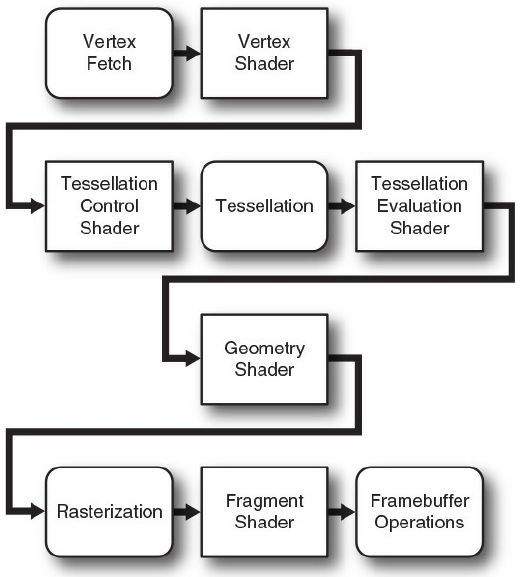
\includegraphics[width=0.75\textwidth]{graphicsPipeline}
	\caption{Упрощенная структура графического конвейера}%
    \label{fig:graphicsPipeline}
\end{figure}
На рисунке~\ref{fig:graphicsPipeline} блоки со скругленными краями представляют
собой фиксированные части, которые обычно реализованы как часть драйвера,
прошивки или другого системного ПО. Блоки с прямоугольными краями являются
программируемыми, это означает, что они могут выполнять шейдеры, предоставляемые
разработчиками ПО.

На момент написания диссертации существует 20 изданий спецификации
OpenGL~\cite{OpenGLHistory}. Номера версий и даты их публикации приведены в
таблице~\ref{table:OpenGLVersions}.
\begin{table}
\caption{Версии OpenGL}%
\label{table:OpenGLVersions}
\centering
\small
\begin{tabular}{| l | l |}
    \hline
    Версия & Дата публикации \\
    \hline
    OpenGL 1.0 & Январь 1992 \\
    OpenGL 1.1 & Январь 1997 \\
    OpenGL 1.2 & Март 1998 \\
    OpenGL 1.2.1 & Октябрь 1998 \\
    OpenGL 1.3 & Август 2001 \\
    OpenGL 1.4 & Июль 2002 \\
    OpenGL 1.5 & Июль 2003 \\
    OpenGL 2.0 & Сентябрь 2004 \\
    OpenGL 2.1 & Июль 2006 \\
    OpenGL 3.0 & Август 2008 \\
    OpenGL 3.1 & Март 2009 \\
    OpenGL 3.2 & Август 2009 \\
    OpenGL 3.3 & Март 2010 \\
    OpenGL 4.0 & Март 2010 \\
    OpenGL 4.1 & Июль 2010 \\
    OpenGL 4.2 & Август 2011 \\
    OpenGL 4.3 & Август 2012 \\
    OpenGL 4.4 & Июль 2013 \\
    OpenGL 4.5 & Август 2014 \\
    OpenGL 4.6 & Октябрь 2017 \\
    \hline
\end{tabular}
\end{table}
Старые версии OpenGL предлагали непосредственный режим работы (фиксированный
конвейер), который был простым способом для отрисовки графики.
Однако, большинство функционала было спрятана в библиотеке и у разработчиков не
было большого контроля над вычислениями. Начиная с версии 3.2 спецификации
началось стимулирование перехода разработчиков к новому API (core профиль),
который является версией спецификации, в которой убрана вся устаревшая
функциональность. Начиная с версии 3.3 радикальных изменений в спецификации не
происходило, в последующих версиях были добавлены некоторые функции для более
удобного выполнения частых задач. Разработанная в ходе диссертации система
использует спецификацию OpenGL версии 4.5, однако может быть легко портирована и
на более ранние версии.

Необходимо вернуться к обзору графического конфейера и дать определение понятию
''шейдер''. \textbf{Шейдеры} --- это небольшие программы, которые предназначены
для выполнения на графическом процессоре~\cite{LearnOGL}. Шейдеры могут
одновременно выполняться на тысячах вычислительный ядер ГП. Для вывода
изображения на экран необходимо наличие в шейдерной программе как минимум
вершинного и фрагментного шейдеров. Для написания шейдеров на OpenGL
используется \textbf{OpenGL Shading Language (GLSL)}. GLSL\@--- Си-подобный язык,
который также является частью спецификации OpenGL\@.

Одну из особенностей OpenGL является использование пяти различных координатных
систем:
\begin{itemize}
    \item локальное пространство (или пространство объекта);
    \item мировое пространство;
    \item пространство наблюдателя;
    \item пространство отсечения;
    \item экранное пространство.
\end{itemize}

Для преобразования координат из одного пространства в другое,
используется несколько различных матриц трансформации, среди которых, самыми важными
являются матрицы модели, вида и проекции. Координаты вершин появляются в
локальном пространстве как локальные координаты, и в дальнейшем преобразуются в
мировые координаты, потом в координаты вида, отсечения, и, наконец, все
все координаты приводятся к экранному пространству. На
рисунке~\ref{fig:spaceTransforms} представлена вся последовательность
преобразований и эффект, который оказывает каждое преобразование:
\begin{figure}[htb]
	\centering
	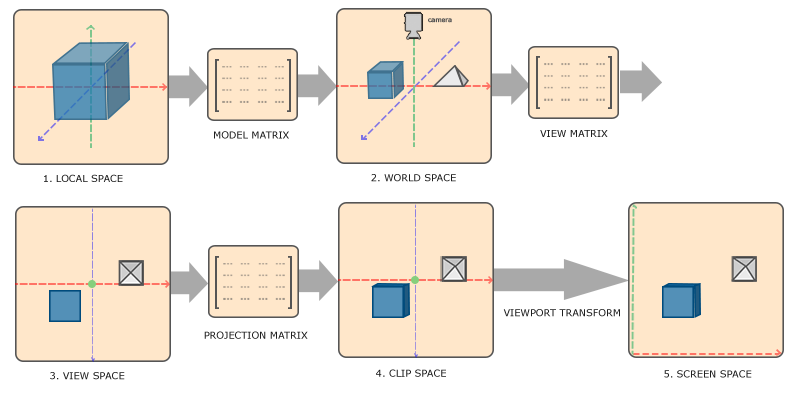
\includegraphics[width=\textwidth]{spaceTransforms}
	\caption{Преобразования систем координат в OpenGL}%
    \label{fig:spaceTransforms}
\end{figure}
\begin{enumerate}
    \item Локальные координаты это координаты объекта измеряемые относительно
        точки отсчета расположенной в центре объекта.

    \item На следующем шаге локальные координаты преобразуются в координаты
        мирового пространства, которое содержит все объекты сцены. Эти
        координаты измеряются относительно глобальной точки отсчета, единой для
        всех объектов расположенных в мировом пространстве.

    \item Далее происходит преобразование мировых координаты в координаты
        пространства наблюдателя таким образом, что каждая вершина становится
        видна как если бы на нее смотрели из камеры или из местоположения
        наблюдателя.

    \item После того, как координаты были преобразованы в пространство
        наблюдателя, необходимо спроецировать их в координаты пространства
        отсечения. Координаты пространства находятся в диапазоне от -1.0 до 1.0
        и определяют, какие вершины появятся на экране.

    \item И, наконец, происходит преобразование координат в экранное
        пространство. Размер пространства определяется размером окна, в котором
        происходит рендеринг изображения. В качестве точки отсчета берется
        нижний левый угол окна. Полученные координаты отсылаются растеризатору
        для превращения их во фрагменты (пиксели).
\end{enumerate}

Операцию приведения координат из пространства в модели в пространство отсечения
можно выполнить с помощью формулы (\ref{eq:mvp}).
\begin{equation}
  \label{eq:mvp}
  \text{V}_\text{clip} = \text{M}_\text{proj} \cdot \text{M}_\text{view} \cdot
  \text{M}_\text{model} \cdot \text{V}_\text{local}
\end{equation}
\begin{explanationx}
    \item [где] $\text{V}_\text{clip}$ --- координаты вершины в пространстве
        отсечения;
    \item $\text{M}_\text{proj}$ --- матрица преобразования в пространство
        отсечения;
    \item $\text{M}_\text{view}$ --- матрица преобразования в пространство
        наблюдателя;
    \item $\text{M}_\text{model}$ --- матрица преобразования в мировое
        пространство;
    \item $\text{V}_\text{local}$ --- координаты вершины в локальном
        пространстве.
\end{explanationx}

Матрицы не обладают свойством коммутативности, поэтому важно выполнять умножение
в правильном порядке. Умножение матриц следует читать в обратном порядке,
т\@.к\@. сначала к вершине применяется самая правая операция.

\section{Физика огня}

Перед тем, как приступить к симуляции огня, нужно глубже разобраться в природе
исследуемого объекта. Необходимо выделить разницу между огнем и пламенем,
дать определение процессу горения и описать его компоненты, сделать обзор
основных видов огня и глубже разобраться в физике процесса горения.

\subsection{Компоненты горения}

В русском языке нет четкого смыслового разделения слов пламя и
огонь\break{}\cite{WikiFlame}, однако в зарубежной литературе присутствует четкое
разделение понятий огонь (fire) и пламя (flame).

Несмотря на то, что стандарт СТ СЭВ 383--87~\cite{383-87} уже устарел, в нем
дается точное определение для ключевых терминов, используемых в диссертации. В
следующих подразделах также будут приведены определения из данного стандарта.

\textbf{Огонь} --- процесс горения, сопровождающийся пламенем или свечением.

\textbf{Пламя} --- зона горения в газовой фазе с видимым излучением.

Среди процессов химических веществ бывают случаи, когда вещество сгорает без
пламени~\cite{WikiFire}.

Обычно люди воспринимают горящий объект, словно горит сам объект. Однако, на
самом деле горит не сам объект, а топливо, которое он выделяет в окружающую
среду. Топливо подымается над поверхностью объекта из-за тепла, испаряется,
вступает в контакт к кислородом и воспламеняется. Таким образом, огонь нуждается
в совместном присутствии трех элементов: топливо, тепло и
кислород~\cite{USArmy}:
\begin{enumerate}
    \item \emph{Топливо}. Топливом может быть твердая, жидкая либо газообразная
        субстанция, также топливо должно химически разлагаться на газы или
        пар. Процесс разложения происходит под воздействием тепла.
    \item \emph{Тепло}. Тепло --- это мера молекулярной активности в объекте,
        увеличение температуры ведет к увеличению скорости движения молекул.
        Если к объекту приложено достаточно тепла, молекулы начинают двигаться
        настолько быстро, что могут покидать поверхность объекта. Так происходит
        процесс перехода топлива в газообразное состояние.
    \item \emph{Кислород}. Кислород является окисляющим агентом и поэтому
        необходим для процесса горения. На определенном уровне, частицы огня
        могут превращаться в частицы дыма из-за нехватки кислорода в воздухе,
        что вызывает неполное окисление.
\end{enumerate}

\section{Воспламенение объектов}

\textbf{Горение} --- экзотермическая реакция окисления вещества,
сопровождающаяся по крайней мере одним из трех факторов: пламенем, свечением,
выделением дыма~\cite{383-87}.

Процесс горения имеет следующие стадии:
\begin{enumerate}
    \item Окисление вызывает разложение горючего материала, происходит \break{}
        медленное выделение газов, включая водяной пар.  Процесс протекает
        непрерывно все время, в течение которого объект взаимодействует с
        окисляющим агентом, которым может выступать воздух.  При температуре
        окружающей среды окисление обычно происходит настолько медленно, что
        даже незаметно человеку. Горючие газы пока еще не могут воспламенятся на
        этой стадии.

    \item Скорость окисления возрастает с ростом температуры, в это время
        некоторые газы становятся воспламеняемыми. Точка, когда в воздухе
        находится достаточное количество пара, чтобы создать горючую смесь в
        воздухе, называется \emph{точкой вспышки}.

    \item В вышеупомянутой точке в выделенных газах присутствует слишком много
        углекислого газа и водяного пара, чтобы поддерживать пламя
        продолжительное время. Однако, тепло огня служит началом для вторичного
        процесса разложения, которое приводит к процессу устойчивого горения.
        Эта точка называется \emph{точкой воспламенения}, и она обычно находится
        на несколько градусов выше точки вспышки.

    \item Окисление может идти настолько быстро, что оно покрывает всю
        поверхность топлива и блокирует доступ к кислороду, препятствуя горению
        топлива и затрудняя проникновение тепла. Это задерживает распространение
        температуры возгорания вглубь горючего материала. Однако, с увеличением
        температуры топливо начинает светиться, воздух поступает внутрь для
        поддержания горения, и происходит горение топлива совместно с
        выделяемыми газами.

    \item Если тепла выделяется больше, чем теряется из-за проводимости,
        конвекции или излучения, огонь будет поддерживаться и появится пламя.
        Горение будет поддерживаться, пока либо тепло, горючее, или окисляющий
        агент не будут убраны из системы.
\end{enumerate}

\section{Динамическая симуляции огня}

В общем случае задача симуляции огня может быть разбита на три
непересекающихся подзадачи~\cite{Perry94synthesizingflames}:
\begin{itemize}
	\item моделирование;
	\item анимация;
	\item визуализация.
\end{itemize}

В первую очередь необходимо выбрать подходящую внутреннюю структуру, или модель,
для симуляции. Далее, требуется выбрать способ анимации --- метод, с помощью
которого будет происходить взаимодействие с моделью. Техника анимации служит для
того, чтобы оживить модель, привести ее в движение. Наконец, модель и ее
анимацию необходимо отрисовать на экране, используя для этого некоторые
примитивы визуализации (полигоны, текстуры, сферы, воксели и т.п.). В
последующих подразделах будут последовательно рассмотрены каждая из этих стадий,
и их взаимовлияние.

\subsection{Моделирование и визуализация огня}

Стохастические методы моделирования огня, такие как поля турбулентности и шумов
очень эффективны при создании реалистичного огня в 2D графике, но являются
крайне неэффективными по количеству операций для использования в 3D анимациях в
реальном времени, независимо от выбранной техники визуализации. Напротив,
эффективно релизованная объемная модель рендеринга, использующая воксели,
помогает достичь приемлемую для интерактивных приложений частоту кадров. Однако,
при использовании данной модели сложно добиться реалистичных результатов,
поскольку поверхность огня не имеет четких границ. Наиболее быстрым методом
является объемное моделирование с использованием полигонов для визуализации;
отрисовка полигонов происходит крайне быстро, однако полигоны не лучшее средство
для визуализации языков пламени, вихрящегося дыма и частиц сажи, и поэтому
обычно полигоны пораждают довольно грубые и низкокачественные результаты. Где-то
между ними находится моделирование с помощью систем частиц, данный метод может
работать с желаемой скоростью, в зависимости от выбранного масштаба, который
выбирается из расчета необходимого уровня детализации и выбранных техник
анимации и визуализации.
